\documentclass{article}

\usepackage{hyperref}
\usepackage{enumerate}
\usepackage{enumitem}
\usepackage{amssymb,amsmath,amsthm} %must be before unicode-math
\usepackage[mathletters]{ucs}
\usepackage{tikz}
\DeclareUnicodeCharacter{8348}{_t}
\DeclareUnicodeCharacter{8342}{_k}
\DeclareUnicodeCharacter{8339}{_x}
\DeclareUnicodeCharacter{8345}{_n}
\DeclareUnicodeCharacter{7522}{_i}
\DeclareUnicodeCharacter{11388}{_j}
\DeclareUnicodeCharacter{8344}{_m}
\DeclareUnicodeCharacter{7523}{_r}
\DeclareUnicodeCharacter{7580}{^c}
\DeclareUnicodeCharacter{7496}{^d}
\DeclareUnicodeCharacter{7511}{^t}
\DeclareUnicodeCharacter{7503}{^k}
\DeclareUnicodeCharacter{7488}{^T}
\DeclareUnicodeCharacter{8346}{_p}
\DeclareUnicodeCharacter{7493}{^\alpha}
\usepackage[utf8x]{inputenc}
\usepackage{graphicx}
\usepackage{stmaryrd}
\usepackage[autosize]{dot2texi}
\usepackage{multicol}
\setlength{\multicolsep}{0pt}
\usepackage{tikz}
\usetikzlibrary{shapes,arrows,tikzmark,decorations.pathreplacing,calc}
\usepackage{adjustbox}

% Title portion. Note the short title for running heads

\title{Piecewise affine approximation of smooth algebraic subvariety of the
projective space in any dimension and codimension}
\author{Christophe Raffalli}

\newcommand{\interior}[1]{%
  #1^{\mathrm{o}}%
}
\newcommand{\cardinal}[1]{%
  \#({#1})%
}
\newcommand{\hull}[1]{%
  \mathcal H({#1})%
}
\newcommand{\nhull}[2]{%
  \mathcal H^\nabla({#1},{#2})%
}
\newcommand{\cone}[1]{%
  \mathcal C({#1})%
}
\newcommand{\ncone}[2]{%
  \mathcal C^\nabla({#1},{#2})%
}
\newcommand{\vertices}[1]{%
  \mathcal V({#1})%
}
\newcommand{\ball}[2]{%
  \mathcal B_{#2}({#1})%
}
\newcommand{\cball}[2]{%
  \mathcal Bᶜ_{#2}({#1})%
}

\newcommand{\PNR}{{\cal P}^n(ℝ)}
\newcommand{\SNR}{{\cal S}^n(ℝ)}
\newcommand{\sgn}{\mathrm{sgn}}

\newtheorem{theo}{Theorem}
\newtheorem{coro}[theo]{Corollary}
\newtheorem{nota}[theo]{Notation}
\newtheorem{defi}[theo]{Definition}
\newtheorem{prop}[theo]{Proposition}
\newtheorem{exam}[theo]{Example}
\newtheorem{lemm}[theo]{Lemma}


% Document starts
\begin{document}

\maketitle

\tableofcontents

\section{Introduction}

\begin{figure}
  \begin{center}
    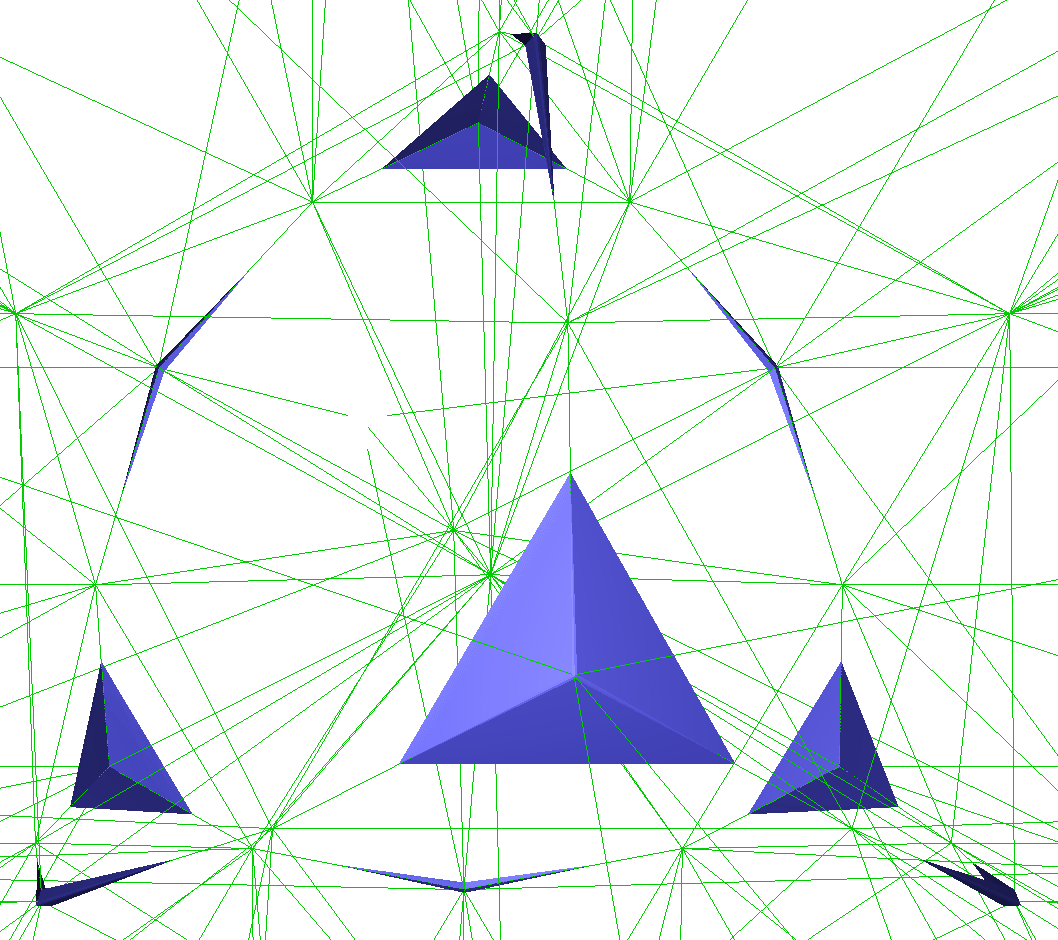
\includegraphics[width=\linewidth]{quartic-M-2.png}
    \caption{piecewise linear approximation of a quartic surface}
  \end{center}
\end{figure}

We present an algorithm solving smooth systems of homogeneous polynomial
equations $\{x ∈ \PNR, p₁(x) = 0, \dots, pₖ(x) = 0\}$. By \emph{smotth},
we mean than the vectors $(∇p₁(x),\dots,∇pₖ(x))$ are linearly independant for
all $x$. By
\emph{solving} we mean finding a piecewise linear approximation of the
solution that is homeomorphic to the real solution allowing for instance to
compute topological invariants of the solution and in particular the number of
connected components. We therefore do not limit ourselves to the zero
dimensional case.

To obtain the solution, we partition the projective space $\PNR$ is a
family of simplices $(Δⱼ)_{j∈J}$, then we construct
the piecewise linear functions $\overline{p}ᵢ$ that are linear on each $Δⱼ$ and
coincide with $pᵢ$ on the vertices of the simplices $Δⱼ$.

Then, we give a criteria to ensure that the set $\{x ∈ \PNR,
\overline{p}₁(x) = 0, \dots, \overline{p}ₖ(x) = 0\}$ is homeomorphic to the
solution of the original system.

The criteria can be summarised as follows:
\begin{itemize}
  \item For each point $x$ of $\PNR$, consider the set of simplices $\{Δ_{j₁},
    \dots, Δ_{jₘ}\} = \{Δⱼ, x ∈ Δⱼ\}$.
  \item For each polynomial $pᵢ$, this gives a set of $m+1$ vector: the gradient
    of the original polynomial $pᵢ$ at $x$, and the gradient of each linear
    function ${\overline{p}ᵢ}_{\restriction Δ_{jₖ}}$ at $x$:
    $$Gᵢ(x) = \{∇pᵢ(x),∇{\overline{p}ᵢ}_{\restriction Δ_{j₁}}(x),  \dots,
      ∇{\overline{p}ᵢ}_{\restriction Δ_{jₘ}}(x)\}$$
    \item Then the criteria is satisfied if for any $x \in \PNR$ such that ...
      and for any
      $(ε₁,\dots,εₖ) ∈ \{-,+\}ᵏ$, $0$ is not in the convex hull of
      $ε₁ G₁(x) ∪ \dots ∪ εₖ Gₖ(x) $.
\end{itemize}

This gives the spirit of the criterion. The real criterion needs a bit more care
as gradient of polynomials are not well defined
This criteria can be checked in practice with a sufficient condition as precise
as we want (up to more computation) using the fact that polynomials written in
the Berstein bases are in the convex hull of their coefficients.

The part of the algorithm is to construct a partition of $\PNR$ that satisfy the
above criterion. We are not yet able to prove that this part of our algorithm
terminates. But it does terminate in practice. It even seem that it requires a
partition whose size is bounded by a constant that only depends upon the number
of variables, number of polynomials and their degree (see conjecture \ref{?}).

Is important to remark that the correction of the algorithm only requires the
criterion to be proved correct, which is done in that paper.

%<!-- Local IspellDict: british -->
%<!-- Local IspellPersDict: ~/.ispell-british -->

\section{Conventions and notations}

We consider the real projective plane $\PNR$.
 We define $πₙ:ℝ^{n+1}∖\{0\} → \PNR$ the
projection $x ↦  \{ λx, λ∈ℝ^⋆ \} ∈ \PNR$. To simplify, we often write $\overline{x}$ for $πₙ(x)$.


We use on $\PNR$ the measure and topology induced by
the chord metric of the unit sphere:
$$d(\overline{x},\overline{y}) = \min\left(
\left\|{\frac{x}{\|x\|}} - {\frac{y}{\|y\|}}\right\|, \left\|{\frac{x}{\|x\|}} + {\frac{y}{\|y\|}}\right\|\right) (∀\overline{x},\overline{y} ∈ \PNR).$$

If $x ∈ \PNR$ (resp. $ℝ^{n+1}$), $\ball{x}{r}$ denotes the open ball of center $x$
and radius $r$ and $\cball{x}{r}$ denotes its closure.

We write $\cardinal{S}$ the cardinal of a set $S$.

For $A ⊂ ℝ^{n+1}$, $\hull{A}$ denotes the convex hull of $A$ and $\cone{A}$ its
convex cone:
$$\cone{A} = \{ ∑_{i=0}ⁿ λᵢ xᵢ, x₀,\dots,xₙ ∈ A, λ₀,\dots,λₙ∈ℝ^⋆₊\}$$
$$\hull{A} = \{ ∑_{i=0}ⁿ λᵢ xᵢ, x₀,\dots,xₙ ∈ A, λ₀,\dots,λₙ∈ℝ^⋆₊,
∑_{i=1}ⁿ λᵢ=1 \}$$

We use the following notation for closed simplices:
\begin{itemize}
\item If $Δ ⊂ \PNR$ is a closed simplex, we denote $\vertices{Δ} ⊂ \SNR$ a finite set of
  representatives of the vertices of $Δ$.
\item $\vertices{Δ}$ must verify that $Δ = πₙ(\hull{\vertices{Δ}})$. This is why we take $\vertices{Δ} ⊂
    \SNR$ instead of $\vertices{Δ} ⊂ \PNR$ as the convex hull is not well defined in
    the projective plane.
\item Simplices should not be too big, in particular, $\PNR$ is not a simplex!
  For this we require $\vertices{Δ}$ to fit in an open half space of
  $\SNR$. If this is not possible, we consider that $Δ$ is not a simplex.
\item We take $\vertices{Δ}$ to be minimal and consider only non degenerated simplex: removing one point in
    $\vertices{Δ}$
    changes it convex hull and the dimension of the
    simplex $Δ$ is always exactly $\cardinal{\vertices{Δ} - 1}$. This also means that
    $\vertices{Δ}$ is the set of extremal points of its convex hull.
  \item Because we require simplices to be not too big $πₙ^{-1}(Δ)$ has exactly two connected components:
    $$πₙ^{-1}(Δ) = \cone{\vertices{Δ}} ∪ -\cone{\vertices{Δ}}.$$
    We write $Δ⁺ =  \cone{\vertices{Δ}}$ and $Δ⁻ = - Δ⁺$. Here $-A$ denotes
    $\{-x, x ∈ A\}$.

\end{itemize}

%<!-- Local IspellDict: british -->
%<!-- Local IspellPersDict: ~/.ispell-british -->

\section{Simplicial partition}

\begin{defi}
  A \emph{simplicial partition} of
  $\PNR$ is a finite set of closed simplices $(Δᵢ)_{i∈I}$ such that
  \begin{itemize}
  \item Each $Δᵢ$ is a simplex of dimension $n$, i.e. $\cardinal{\vertices{Δ}} = n + 1$.
  \item $⋃_{i∈I} Δᵢ = \PNR$,
  \item For all $i₁ < i₂ < \dots iₖ ∈ I$, $Δ_{i₁} ∩ \dots ∩ Δ_{iₖ}$ is empty or is a simplex of dimension at most
    $n-k+1$ and $πₙ(\vertices{Δ_{i₁} ∩ \dots ∩ Δ_{iₖ}}) =
    πₙ(\vertices{Δ_{i₁}}) ∩ \dots ∩ πₙ(\vertices{Δ_{iₖ}})$.
    We can not require  $\vertices{Δᵢ ∩ Δⱼ} = \vertices{Δᵢ} ∩ \vertices{Δⱼ}$ because we may have $x ∈
    \vertices{Δᵢ}$ and $y ∈ \vertices{Δⱼ}$ with $x ≠ y$ and $\overline{x} = \overline{y}$ (see
    the example below). This conditions ensures that the intersection of
    simplices consists exactly in the face of lower dimensions defined by the
    common vertices of the simplices.
%  \item We say that $Δᵢ$ and $Δⱼ$ are neighbour if $Δᵢ ∩ Δⱼ ≠ ∅$. The neighbourhood relation is clearly reflexive and symmetric.
  \end{itemize}
\end{defi}

Here is as example a partition of $\PNR$ with $2ⁿ$ simplices:
\begin{exam}\label{init_part}
Consider $B = \{x₀,\dots,xₙ\}$, the canonical base of $ℝ^{n+1}$ and
$(εᵢ)_{i ∈ \{1,\dots,2ⁿ\}}$ an enumeration of all sequences of length $n$ of
$1$ or $-1$. Then, we define $(Δᵢ)_{i∈\{1,\dots,2ⁿ\}}$ by
$$Δᵢ = πₙ(\hull{\{x₀,ε_{i,1} x₁, \dots, ε_{i,n} xₙ\}}).$$
\end{exam}

We remark in this example, that all simplices use $B$ as set of vertices. This
means that for all $i < j ∈ \{1,\dots,2ⁿ\}$, we have
  $πₙ(\vertices{Δᵢ}) = πₙ(\vertices{Δⱼ}) = πₙ(B)$ while $\vertices{Δᵢ} ≠ \vertices{Δⱼ}$.

In this examples, we have
\begin{eqnarray*}
  Δ⁺ᵢ &=& \cone{\{x₀,ε_{i,1} x₁, \dots, ε_{i,n} xₙ\}} \cr
  Δ⁻ᵢ &=& \cone{\{-x₀,-ε_{i,1} x₁, \dots, -ε_{i,n} xₙ\}} \cr
\end{eqnarray*}

\begin{defi} Let $(Δᵢ)_{i∈I}$ be a simplicial partition of $\PNR$. For $x ∈
  ℝ^{n+1} ∖\{0\}$ we define
  $I^Δ(x) = \{(i,σ) ∈ I × \{-,+\}, x ∈ Δᵢ^σ\}$. In general we only use one
  simplicial partition at a time and we simply write $I(x)$.
\end{defi}

\begin{prop}\label{Ihomo}
  Let $(Δᵢ)_{i∈I}$ be a simplicial partition of $\PNR$.
  For $x ∈  ℝ^{n+1} ∖\{0\}$ and $λ > 0$, we have $I(λx) = I(x)$.
\end{prop}

\begin{proof}
  From the fact that the set $Δᵢ^σ$ are convex cones.
\end{proof}

%<!-- Local IspellDict: british -->
%<!-- Local IspellPersDict: ~/.ispell-british -->

\section{Δ-linear approximation of a polynomial}

\begin{defi}
Let $p$ be an homogeneous polynomial of degree $d$ on
$ℝ^{n+1}$. Let $(Δᵢ)_{i∈I}$ be a simplicial partition of $\PNR$.
We define $\overline{p} : ℝ^{n+1} → ℝ$, the \emph{$Δ$-linear approximation of $p$},
the piecewice linear function
that is linear on all $Δ^σᵢ$ for $i ∈ I$, $σ ∈ \{+,-\}$, and equal to $p$
on all points in $\vertices{Δ}$.

For $i ∈ I$, $σ ∈ \{+,-\}$, we define $∇ᵢ^σp = ∇\overline{p}(x)$
for any $x ∈ Δ^σᵢ$, as the gradient is constant over $Δ^σᵢ$ for a linear
function.

We also define $\hat p(x) = \sgn(\overline{p}(x))^{d-1} \overline{p}^d(x)$. $\hat p$
is homogeneous of degree $d$, i.e. for $x \in ℝ^{n+1}$ and $λ>0$, $\hat p(λx) = λᵈ
\hat p(x)$. The function $\overline{p}$ and $\hat p$ obviously have the same sign and
zero locus on $ℝ^{n+1}$.
\end{defi}

\begin{lemm}
Let $p$ be an homogeneous polynomial of degree $d$ on
$ℝ^{n+1}$. Let $(Δᵢ)_{i∈I}$ be a simplicial partition of $\PNR$.
The function $\overline{p}$ and $\hat p$ have derivatives at $x ∈ ℝ^{n+1} ∖\{0\}$ in the
direction $v$ if the point $I(x + h v)$ is constant
for $h ∈ [-ε,ε]$ with $ε > 0$ is small enough.

This means that for any line segment $\overline{p}$ and $\hat p$ have
derivatives almost everywhere in the direction of this line.
\end{lemm}

\begin{proof}
  Lines can only meet transversaly intersections $πₙ^{-1}$ of the intersection
  of at least two simplices of $Δ$ in finitely many points.
\end{proof}

\begin{lemm}
  From the previous lemma, with the same hypothesis, we find that $\hat p$ is
  Lipschitz in $\ball{0}{M}$ for any $M ∈ ℝ₊$.
\end{lemm}

\begin{proof}
  Let $L$ be the maximum of the differential of $\hat p$, where it is defined in
  $\ball{0}{M}$. At a point $x$ in $D = \ball{0}{M} ∩ πₙ^{-1} (Δ_{i₁} ∩ \dots ∩
  Δ_{iₖ})$, if $v$ is a direction tangent to this intersection, then $\nabla
  \hat p_{i₁}(x) . v = \dots = \nabla \hat p_{iₖ}(x) . v$ because the functions
  $\hat p_{i₁}, \dots, \hat p_{iₖ}$ coincide on $D$. We will denote this number
  by $\nabla \hat p(x) . v$, which for $v$ fixed is defined almost every where,
  and we have $\nabla \hat p(x) . v ≤ \min_{j ∈ (i₁,\dots,iₖ)} \|\nabla \hat
  pⱼ(x)\| \|v\| ≤ L \|v\|$.

  Then, we have
  \begin{eqnarray*}
    |\hat p(x) - \hat p(y)| &=& \left. ∫₀¹ \nabla \hat p(x + (1-t) y) . (x - y)
    dt\right. \cr
    &≤&   ∫₀¹ L \|(x - y)\| dt \cr
    &≤& L \|x - y\|
  \end{eqnarray*}
\end{proof}

\begin{defi}
Let $p$ be an homogeneous polynomial of degree $d$ on
$ℝ^{n+1}$. Let $(Δᵢ)_{i∈I}$ be a simplicial partition of $\PNR$.
Let $\overline{p}$ be the $Δ$-linear approximation of $p$.
We define
\begin{itemize}
  \item the condition $Π_p(x)$ to be true if and only if $p(x)$ and
$\overline{p}(x)$ are both positive or both negative (i.e. $p(x)
    \overline{p}(x) > 0$),
  \item The set $\ncone{p}{x} = \cone{\{∇p(x)\} ∪ \{∇ᵢ^σp, (i,σ) ∈ I(x)\}}$
  \item The set $\nhull{p}{x} = \hull{\{∇p(x)\} ∪ \{∇ᵢ^σp, (i,σ) ∈ I(x)\}}$
\end{itemize}
\end{defi}

\begin{prop}\label{adaptedeq}
Let $p$ be an homogeneous polynomial of degree $d$ on
$ℝ^{n+1}$. Let $(Δᵢ)_{i∈I}$ be a simplicial partition of $\PNR$.
Let $\overline{p}$ be the $Δ$-linear approximation of $p$.

The following conditions are equivalent:
\begin{enumerate}
\item $∀x ∈  ℝ^{n+1}∖\{0\}, Π_p(x) \hbox{ or } 0 ∉ \ncone{p}{x}$
\item $∀x ∈  ℝ^{n+1}∖\{0\}, Π_p(x) \hbox{ or } 0 ∉ \nhull{p}{x}$
\item $∀x ∈  \SNR, Π_p(x) \hbox{ or } 0 ∉ \ncone{p}{x}$
\item $∀x ∈  \SNR, Π_p(x) \hbox{ or } 0 ∉ \nhull{p}{x}$
\item\label{hb} $∀x ∈  ℝ^{n+1}∖\{0\}, Π_p(x) \hbox{ or } ∃δ ∈ ℝ^{n+1}∖\{0\},
  \left\{\begin{array}{l} δ.∇p(x) > 0 \hbox{ and}\cr
    ∀(i,σ) ∈ I(x), δ.∇ᵢ^σp > 0
  \end{array}\right.$
\end{enumerate}
\end{prop}

\begin{proof}
  The equivalences (1) ↔ (2) and (3) ↔ (4) are a general property of convex hull
  and convex cone: for any set $X ⊂ ℝ^{n+1}$, $0 ∈ \hull{X} ↔ 0 ∈ \cone{X}$.
  %Left to right is because $\hull{X} ⊆ \cone{X}$. For right to left, if $0 ∈
  %\cone{X}$, if means we write $0 = λᵢ x₁ + \dots + λₙ xₙ$ with $λᵢ > 0$ and
  %$xᵢ ∈ X$ for $1 < i < n$. Hence, taking $μᵢ = \frac{λᵢ}{λᵢ + \dots + λₙ}$, we
  %have $0 = μᵢ x₁ + \dots + μₙ xₙ$ with $μ₁ + \dots + μₙ = 1$ and $μᵢ > 0$, $xᵢ
  %∈ X$ for $1 < i < n$.


  The equivalence (1)  ↔ (3) comes from proposition $\ref{Ihomo}$ and the fact that $p$ is homogeneous hence
  $\nabla(p)(λx) = λ^{d-1}\nabla(p)(x)$ for $λ > 0$.

  The equivalence (2) ↔ (5) is a form of Han-Banach theorem ensuring the
  existence of a supporting hyper-plane for points outside a convex body. The
  vector $δ$ is a normal vector of this supporting hyperplane \cite{Zal02}.
\end{proof}

\begin{defi}
Let $p$ be an homogeneous polynomial of degree $d$ on
$ℝ^{n+1}$. Let $(Δᵢ)_{i∈I}$ be a simplicial partition of $\PNR$.
We say that the partition is \emph{adapted} to $p$ if it satisfies the conditions
of proposition \ref{adaptedeq}.
\end{defi}

\begin{coro}
  Let $p$ be an homogeneous polynomial of degree $d$ on
  $ℝ^{n+1}$. Let $(Δᵢ)_{i∈I}$ be a simplicial partition of $\PNR$ adapted to $p$.
  Then, the zero-locus of $p$ and $\overline{p}$ the $\Delta$ approximation of
  $p$ are isomorphic.
\end{coro}

This theorem is a consequence of the theorem \ref{maintheo} to come.

\begin{defi}
Let $p_1,\dots,p_k$ be $k$ homogeneous polynomial of degree $d_1,\dots,d_k$ on
$ℝ^{n+1}$. Let $(Δᵢ)_{i∈I}$ be a simplicial partition of $\PNR$.

We say that the partition is \emph{adapted} to $p_1,\dots,p_k$ if it satisfies
the following condition: for all $x \in ℝ^{n+1}$, either $\Pi_{p_j}(x)$ is true
for some $1 \leq j \leq k$ or $\ncone{p₁}{x} × \dots × \ncone{pₖ}{x}$ contains
only linear independant tuple of vectors.
\end{defi}

\begin{theo}\label{maintheo}
  Let $p_1,\dots,p_k$ be $k$ homogeneous polynomial of degree $d_1,\dots,d_k$ on
$ℝ^{n+1}$. Let $(Δᵢ)_{i∈I}$ be a simplicial partition of $\PNR$ adapted to
  $p₁,\dots,pₖ$. Then, the zero locus of $p₁,\dots,pₙ$ is isomorphic to the zero
  locus of $\overline{p}₁,\dots,\overline{p}ₖ$.
\end{theo}

We will prove our main theorem is the next two sections. The rest of the paper
explains how to test that a simplicial partition is adapted to a finite set of
polynomials.

%<!-- Local IspellDict: british -->
%<!-- Local IspellPersDict: ~/.ispell-british -->

\section{A variation on Cauchy-Lipschitz theorem}

To prove our main theorem we need a theorem of existence and uniqueness
of solutions for ordinary differential equations that accepts non continuous
function for $t=0$. Here is our lemma:

\begin{lemm}
  Let $Ω$ be an open set of $\SNR$ for the topology of the sphere.
  Let $f$ be a
  function in $]0,1] × Ω → ℝ^{n+1}$ such that $f(t,x)$ is tangent to $\SNR$ at $x$. We assume that $f$ is $(L,α)$-Lipschitz for
  some $L > 0$ and $α ≥ 0$ which we define by:

  \begin{enumerate}
  \item $f$ is continuous and bounded on $]0,1] × Ω$,
  \item $∀t ∈ ]0,1], ∀x,y ∈ Ω, \|f(t,x) - f(t,y)\| ≤ \frac{L}{tᵅ} \|x - y\|$ and
  \end{enumerate}

  Then, the differential equation
  \begin{eqnarray}
    x'(t) = f(t,x(t)) \label{lipschitz-diffeq}
  \end{eqnarray}
  has unique maximal for any initial condition $x(t₀) = x₀ ∈ Ω$
  with $t₀ ∈ [0,1]$. This solutions are of class ${\cal C}¹$.

  Moreover, if we can prove that a solution can't converge to a point outside
  $Ψ$, then this solution is total, i.e. defined on $[0,1]$.
\end{lemm}

\begin{proof}

We remark that if $f$ is $(L,α)$-Lipschitz on $[0,1] × Ω$ then it
is $\frac{L}{tᵅ}$-Lipschitz on $[t,1] × Ω$ for any $t ∈ ]0,1[$.

This proves by the standard Cauchy-Lipschitz result that for any initial condition
$x(t₀) = x₀ ∈ Ω$ with $t₀ ∈ ]0,1]$, we have a unique solution on $[t,1]$ for
    any $0 < t < t₀$ and therefore a unique maximal solution.

    It remains to show that the solution is of class ${\cal C}¹$ even in $0$.
    If a maximal solution is defined on $]0,b]$, then by compacity and because
        $f(t,x)$ is bounded, both $x(t)$ and $x'(t)$ have limits for $t=0$ (this
        limit may be outside of $Ψ$).  The limit of the latter is the derivative
        of $x$ in $0$ by the usual result on the limit of derivatives.
        We do not have that $x'(0) = f(0,x(0))$ as $f$ is not even defined in $0$.

It remains to show the existance and unicity of solutions for initial conditions
in $0$.

We define $n₁(t) = t^{2L}$ and $n_α(t) = e^{-\frac{2L}{α-1} t^{1-α}}$ when $α >
1$. In all cases, we have $n(t) → 0$ when $t → 0$ and $n'_α(t) = \frac{2L}{tᵅ}
n_α(t)$. Indeed:
\begin{itemize}
\item For $α = 1$, $n'₁(t) = 2L t^{2L-1} = \frac{2L}{t} n₁(t)$
\item For $α ≥ 0, α≠ 1$, $n'_α(t) = 2L t^{-α} e^{- \frac{2L}{α-1} t^{1-α}} = \frac{2L}{tᵅ} n_α(t)$
\end{itemize}

Then, we define the
following norms on the set of continuous, partial functions from $[0,1]$ to $Ω$:
$$\|x\|_α = \max_{t ∈ ]
0,1], x(t) \rm defined} \frac{\|x(t)\|}{n_α(t)}$$

Remark: if $\|x\| = 0$ and $x(0) ≠ 0$ then, as $x$ is continuous, we can find $t
> 0$ such that $x(t) > \frac{x(0)}{2}$, hence $\|x\|_α >
\frac{x(0)}{2 n_α(t)}$ which is a contradiction. Therefore, $\|.\|_α$ is indeed
a norm.


We assume that the initial condition of the differential equation
\ref{lipschitz-diffeq} is
$x(0) = x₀ ∈ Ω$.
We define the following operator on continuous partial function from $[0,1]$ to
$Ω$:
$$F(x)(t) = x₀ + ∫^t_0 f(u,x(u)).{\rm d} u$$

For any $t ∈ ]0,1]$, we have:
\begin{eqnarray*}
  \|F(x)(t) - F(y)(t)\| &≤& ∫^t_0 \|f(u,x(u)) - f(u,y(u))\| {\rm d} u \cr
  &≤& ∫^t_0 \frac{L}{uᵅ} \|x(u) - y(u)\| {\rm d} u \cr
  &≤& \|x - y\|_α ∫^t_0 \frac{L}{uᵅ} n_α(u)  {\rm d} u \cr
  &≤& \|x - y\|_α ∫^t_0 \frac{1}{2} n'_α(u)  {\rm d} u \cr
  &≤&\frac{1}{2} \|x - y\|_α n_α(t) \cr
\|F(x) - F(y)\|_α &≤& \frac{1}{2} \|x - y\|_α
\end{eqnarray*}

Therefore, $F$ is
contracting, this ensures the existence and unicity of a fixpoint of $F$, hence
of a solution of the differentiel equation \ref{lipschitz-diffeq} with initial
condition $x(0) = x₀$. Again by compacity and boundedness of $f$ this solution
is of class ${\cal C}¹$.

\end{proof}

%% We choose $s : ℝ^{n+1} → ℝ$, a $C^∞$ function with support in
%% $\ball{0}{1}$ and $∫_{ℝ^{n+1}} s(t) dt = 1$ for the standard measure $dt$
%% on $ℝ^{n+1}$. We will use the same function $s$ in the rest of this paper.

%% \begin{lemm}
%% Let $g$ be a homogeneous continuous function of degree $d$ in $ℝ^{n+1} → ℝ$. We define
%% $f(t,x) = ∫_{ℝ^{n+1}} g(x - t ε u) s(u) {\rm d} u$.
%% Then, $\nablaₓ f$ is L-Lipschitz¹ on $\SNR$.
%% \end{lemm}

%% \begin{proof}
%%   We have
%%   \begin{eqnarray*}
%%     f(t,x) &=& ∫_{ℝ^{n+1}} g(x - t ε u) s(u) {\rm d} u \cr
%%     &=& \frac{1}{(tε)^{n+1}} ∫_{ℝ^{n+1}} g(v) s(\frac{x - v}{tε}) {\rm d} v \cr
%%     \nablaₓ f(t,x) &=&
%%     \frac{1}{(tε)^{n+2}} ∫_{ℝ^{n+1}} g(v) ∇s(\frac{x - v}{tε}) {\rm d} v \cr
%%   \end{eqnarray*}
%% \end{proof}


%<!-- Local IspellDict: british -->
%<!-- Local IspellPersDict: ~/.ispell-british -->

\section{Proof of main theorem}

In this section, we consider that $p₁,\dots,pₖ$ are homogeneous polynomial of
degree $d_1,\dots,d_k$ on $ℝ^{n+1}$ and that $(Δᵢ)_{i∈I}$ is a simplicial
partition of $\PNR$ adapted to $p₁,\dots,pₖ$ and $ε$-thin for some $ε>0$.

We also choose $s:ℝ^{n+1} → ℝ⁺$ a $C^∞$ map with support included in $B_1(0)$
and such that $∫_{ℝ^{n+1}} s(u)du = 1$ for the usual measure $du$ of
$ℝ^{n+1}$. We also assume that $s(-x) = s(x)$.

First, for $t > 0$ and $x ∈ ℝ^{n+1}$, we define $$\hat pⱼ(t,x) = ∫_{ℝ^{n+1}} \hat
pⱼ(x - tεu) s(u)du$$ If we define $fₜ(y) = \hat pⱼ(tεy)$, then $\hat pⱼ(t,x) = (fₜ ⋆
s)(\frac{x}{tε})$ where $fₜ ⋆ s$ denotes the convolution product. Therefore
$\hat pⱼ(t,x)$ is $C^∞$ for its second variable.

We prove a few lemmas about the $\hat pⱼ(t,x)$.

\begin{lemm}[Homogeneity]\label{proof-homogeneity}
  for $t > 0$ and $x ∈ ℝ^{n+1}$, $\hat pⱼ(λt,λx) = λᵈ \hat pⱼ(t,x)$.
\end{lemm}

\begin{proof}
  From the homogeneity of $\hat pⱼ$.
\end{proof}

\begin{lemm}[Derivation]\label{proof-derivation}
  \begin{eqnarray*}
    ∇ₓ pⱼ(t,x) &=& ∇ₓ ∫_{ℝ^{n+1}} \hat pⱼ(x - t ε u)s(u) du \cr
        &=& ∫_{ℝ^{n+1}} ∇\hat pⱼ(x - t ε u) s(u) du \cr
        &=& ∫_{ℝ^{n+1}} ∇\overline pⱼ(x - t ε u) |\overline{pⱼ}^{d-1}(x - tε u)| s(u) du \cr
        &=& d Σ_{(i,σ)∈I_{tε}(x)} ∇ᵢ^σpⱼ. ∫_{\Phiᵢ^σ(x,tε)} |\overline{pⱼ}^{d-1}(x - tε u)| s(u) du\cr
  \end{eqnarray*}

  As the integrals on the last line are positive, this implies that $∇ₓ pⱼ(t,x)$
  is in the convex hull of the vector $∇ᵢ^σpⱼ$ for $(i,σ)∈I_{tε}(x)$.


  \begin{eqnarray*}
    \frac{∂\hat pⱼ(t,x)}{∂t} &=& \frac{∂}{∂t} ∫_{ℝ^{n+1}} \hat pⱼ(x - t ε u)s(u) du \cr
        &=& - ε  ∫_{ℝ^{n+1}} ∇\hat pⱼ(x - t ε u) u s(u) du \cr
        &=& - εd ∫_{ℝ^{n+1}} ∇\overline pⱼ(x - t ε u) |\overline{pⱼ}^{d-1}(x -
    tε u)| u s(u) du \cr
        &=& - εd Σ_{(i,σ)∈I_{tε}(x)} ∇ᵢ^σpⱼ. ∫_{\Phiᵢ^σ(x,tε)} |\overline{pⱼ}^{d-1}(x - tε u)| u s(u) du\cr
  \end{eqnarray*}

  This implies that if $0 < t < \|x\|$ then $\frac{∂\hat pⱼ(t,x)}{∂t} < ε Kⱼ \|x\|^{d-1}$ for some
  constant $Kⱼ > 0$.
\end{lemm}

\begin{lemm}[Limit]\label{proof-limit}
  $$\lim_{t → 0} \hat pⱼ(t,x) = \hat pⱼ(x)$$
  $$\lim_{t → 0} ∇ₓ \hat pⱼ(t,x) =  d Σ_{(i,σ)∈I(x)}
  ∇ᵢ^σpⱼ. |\overline{pⱼ}^{d-1}(x)|  ∫_{\Phiᵢ^σ(x,ε)} s(u) du$$
\end{lemm}

We now consider that $∇ₓ \hat pⱼ(t,x)$ is defined on $[0,1] × ℝ^{n+1}$ using the
above limit for $t = 0$. However $∇ₓ \hat pⱼ(t,x)$ is not in general continuous
in $(0,x)$. Still it is in $∇ₓ \hat pⱼ(t,x) ∈ \ncone{pⱼ}{x}$. We will not really
use $∇ₓ \hat pⱼ(t,x)$ for $t = 0$, but it is more practical if it is defined in
$t = 0$.

\begin{proof}
  \dots
\end{proof}

\begin{lemm}
  Assume $\|x\|<1,\|y\|<1$ and $0 < t ≤ 1$, then we find a constant $L>0$ such that:
  \begin{eqnarray*}
    \|∇ₓ pⱼ(t,x) - ∇_y pⱼ(t,y)\| &=& \left\|∇ₓ ∫_{ℝ^{n+1}} \hat pⱼ(x - t ε u)s(u)
    du - ∇_y ∫_{ℝ^{n+1}} \hat
    pⱼ(y - t ε u)s(u) du \right\| \cr
    &=& \left\|∇ₓ ∫_{ℝ^{n+1}} \hat pⱼ(v)s(\frac{x-v}{tε})\frac{dv}{(tε)^{n+1}} \right.
    \cr
    && \hspace{3em} \left. - ∇_y ∫_{ℝ^{n+1}} \hat
    pⱼ(v) s(\frac{y-v}{tε}) \frac{dv}{(tε)^{n+1}} \right\| \cr
    &=& \left\|∫_{ℝ^{n+1}} \hat pⱼ(v)∇s(\frac{x-v}{tε})\frac{dv}{(tε)^{n+2}} \right.
    \cr
    && \hspace{3em} \left. - ∫_{ℝ^{n+1}} \hat
    pⱼ(v) ∇s(\frac{y-v}{tε}) \frac{dv}{(tε)^{n+2}} \right\| \cr
    &=& \frac{1}{tε} \left\|∫_{ℝ^{n+1}} \hat pⱼ(x - tεu)∇s(u) du
    - ∫_{ℝ^{n+1}} \hat
    pⱼ(y - tεu) ∇s(u) du \right\| \cr
    &≤& \frac{1}{tε} ∫_{ℝ^{n+1}} |\hat pⱼ(x - tεu) - \hat pⱼ(y - tεu)|
    \|∇s(u)\| du \cr
    &≤& L \frac{\|x-y\|}{tε}
  \end{eqnarray*}
\end{lemm}

\begin{defi}
  For $(t,x) ∈ [0,1] × ℝ^{n+1}$, we define
  \begin{itemize}
  \item $Ω$ the compact set defined by $$Ω = \{ x ∈ ℝ^{n+1}, ∀j∈\{1,\dots,k\},
    pⱼ(x) \overline{p}ⱼ(x) ≤ 0 \}$$

  \item $P(t,x)$ the vector in $ℝᵏ$ whose coefficients are
    $$Pⱼ(t,x) = t pⱼ(x) + (1-t) \hat pⱼ(t,x)$$

  \item $G(t,x) = ∇ₓ P(t,x)$ the $(n+1)×k$ matrix whose $k$ columns are the vector
    $$Gⱼ(t,x) = t ∇pⱼ(x) + (1-t) ∇ₓ \hat pⱼ(t,x)$$

  \item $Q(t,x) = \frac{∂P}{∂t}(t,x)$ the vector in $ℝᵏ$ whose coefficients are
    $$Pⱼ(t,x) = pⱼ(x) - \hat pⱼ(t,x) + (1-t) \frac{∂\hat pⱼ}{∂t}(t,x)$$
  \end{itemize}
\end{defi}

\begin{prop}
  The matrix $G(t,x)$ is of rank $k$ for $(t,x) ∈ [0,1] × Ω$ and therefore the
  $k × k$ matrix ${ᵗG}(t,x) G(t,x)$ is invertible.
\end{prop}

\begin{proof}
  From the definition of adapted simplicial partition, we have that the column
  of $G(t,x)$ are linearly independant.
\end{proof}

\begin{defi}
  We define $Gᵀ(t,x)$ the orthogonal projection of $G(t,x)$ on the tangent plane
  to the unit sphere at $x$, column by column.
\end{defi}

\begin{prop}
  We can find $ε$ small enough and a neighbourhood $Ψ$ of $[0,1] × Ω$, open for
  the topology of $[0,1] ×  ℝ^{n+1}$ such that  the matrix $Gᵀ(t,x)$ is still of
  rank $k$ for $(t,x) ∈ Ψ$.
\end{prop}

\begin{proof}
  Using the homogeneity, we get:
  \begin{eqnarray*}
    Gⱼ(t,x).x &=& t ∇pⱼ(x).x + (1-t) (∇ₓ \hat pⱼ(t,x).x) \cr
    &=& t ∇pⱼ(x).x + (1-t) (\frac{∂\hat pⱼ(t,x)}{∂t}, ∇ₓ \hat pⱼ(t,x)).(t, x) -
    t (1-t) \frac{∂\hat pⱼ}{∂}(t,x) \cr
    &=& t d pⱼ(x) + (1-t) d \hat pⱼ(t,x) - t (1-t) \frac{∂\hat pⱼ}{∂t}(t,x) \cr
    &=& d P(t,x)  - t (1-t) \frac{∂\hat pⱼ}{∂t}(t,x) \cr
  \end{eqnarray*}

  For each $x ∈ ...$, the family of matrices in $\nhull{p₁,\dots,pₖ}{x}$ are all
  of rank $k$. This family of matrix is a compact and as $\Delta$ is adapted, it
  is of rank $k$ for any $x ∈ Ω$. Moreover, being of rank $k$ is an open
  condition, therefore we can find a neighbourhood $Ψ$ of $Ω$ and a parameter
  $η$ such that for any  $x ∈ Ψ$ and any $n+1 × k$ matrices $H$ such that $\|G(t,x) - H\| < η$, then we have $H$ of rank $k$.

  Therefore, if $ε$ is small enough and $x ∈ Ψ$ we have $\|G(t,x) - Gᵀ(t,x)\| < η$
  and therefore $Gᵀ(t,x)$ of rank $k$.
\end{proof}

\begin{defi}
  For $x ∈ Ψ$, we define
  $$
  f(t,x) = - Gᵀ(t,x) ({ᵗGᵀ}(t,x) Gᵀ(t,x))^{-1} Q(t,x)
  $$
  and we consider the differential equation $$x'(t) = f(t,x(t))$$
\end{defi}

\begin{prop}
  Let $x : I → Ψ$ be a maximal solution of the above differential equation with
  the initial condition $x(t₀) = x₀$ with $P(t₀,x₀) = 0$. Then, $I = [0,1]$ and
  $P(t,x(t)) = 0$ for all $t ∈ [0,1]$.
\end{prop}

\begin{proof}
  \dots
\end{proof}

%<!-- Local IspellDict: british -->
%<!-- Local IspellPersDict: ~/.ispell-british -->

\section{Implementation details}

%<!-- Local IspellDict: british -->
%<!-- Local IspellPersDict: ~/.ispell-british -->

\section{Conjecture and further work}

%<!-- Local IspellDict: british -->
%<!-- Local IspellPersDict: ~/.ispell-british -->

\appendix
\section{Testing zero in convex hull}

The central test in our algorith is to know if the null vector is in the convex
hull of a given set of vector of $ℝ^d$, or as it is clearly equivalent, in its convex
cone.

More precisely, the problem we want to solve can be defined as follows:
\begin{defi}
  \begin{tabular}{ll}
  Input:& a real $n × d$ matrix $A$. \cr
  Output:& a non nul vector $X ∈ ℝ_+^n$ such that $^tX A = 0$ \cr
  or& a vector $N ∈ ℝ^d$ such that $A N > 0$
  \end{tabular}
\end{defi}

This does correspond to our problem: if zero is in the convex hull of the lines
of the matrix $A$, then we can produce the wanted vector $X∈ ℝ_+^n$. It zero is not in
the convex hull, then we can return the normal $N∈ ℝ^d$ of a linear plane such that
all the lines of $A$ lie on the same side of this plane.

We start the algorithm with an initial vector $X_0∈ ℝ_+^n$, with positive coefficients
summing to one, for instance $X₀=\frac{1}{n}ᵗ(1,1,\dots,1,1)$.
We define $N_i = tX_i A$. We also define a vector $P_0 = 0 ∈ ℝ_+^n $.

The algorithm then perform two kind of steps:

\paragraph*{Conjugate steps}, which are somehow inspired by the conjugate
gradient method.

First we define $J ∈ ℝ_+^n = (1,1,\dots,1,1)$ and $ν(X) = \frac{1}{J.X} X$ which
normalise the vector $X$ to have all its coefficient sum to one. We will use
$ν(X)$ only one non null vector in $ℝ_+^n$.

If for all lines $Aⱼ$ of $A$ we have $Aⱼ.Nᵢ > 0$ then the algorithm
stops and output $N = Nᵢ$. Otherwise we select $Dᵢ = δⱼ$ such that $Aⱼ.Nᵢ ≤ 0$ and minimum.
Then we compute $α>0,β ∈ ℝ$, $X_{i+1} = ν(Xᵢ + αDᵢ+βPᵢ)$, such that
  $\|ᵗX_{i+1} A\|²$ is minimum. We have
  \begin{eqnarray*}
    f(α,β) &=& \|ᵗX_{i+1} A\|² \cr
    &=& \frac{\|ᵗXᵢ A + αᵗDᵢA + βᵗPᵢA\|²}{(1 + α + β)²}\cr
    &=& \frac{\|Nᵢ + αᵗAⱼ + βᵗPᵢA\|²}{(1 + α + βPᵢ.J)²}\cr
    &=& \frac{\|Nᵢ\|² + α² + β²\|ᵗPᵢA\|² + 2 α Nᵢ.Aⱼ + 2 β Nᵢ.ᵗPᵢA + 2αβ Aⱼ.ᵗPᵢA}
    {1 + α² + β²(Pᵢ.J)² + 2α + 2βPᵢ.J + 2αβPᵢJ}\cr
    \frac{∂f(α,β)}{∂α}
    &=& \frac{\begin{array}{cl}
        &(2α + 2 Nᵢ.Aⱼ + 2βAⱼ.ᵗPᵢA)(1 + α² + β²(Pᵢ.J)² + 2α + 2βPᵢ.J + 2αβPᵢJ)\cr
        - &(\|Nᵢ\|² + α² + β²\|ᵗPᵢA\|² + 2 α Nᵢ.Aⱼ + 2 β Nᵢ.ᵗPᵢA + 2αβ
      Aⱼ.ᵗPᵢA)(2α + 2 + 2βPᵢJ)
      \end{array}}{(1 + α² + β²(Pᵢ.J)² + 2α + 2βPᵢ.J + 2αβPᵢJ)²}\cr
    &=&
    {(1 + α² + β²(Pᵢ.J)² + 2α + 2βPᵢ.J + 2αβPᵢJ)²}\cr
  \end{eqnarray*}


\bibliography{main}
\bibliographystyle{plain}

\end{document}

%<!-- Local IspellDict: british -->
%<!-- Local IspellPersDict: ~/.ispell-british -->
